\documentclass[../../Rapport RayTracer.tex]{subfiles}


\begin{document}

Afin de colorer notre scène, nous devons donner une couleur aux formes des objets qui composent la scène. De plus, nous devons indiquer au RayTracer si l'objet est réfléchissant ou si au contraire il est mat, s'il est spéculaire et si oui à quel point, s'il est diffus...
Nous allons donc organiser toutes ces caractéristiques dans ce que l'on va appeler des matériaux.

\begin{figure}[h!]
	\adjustbox{center}{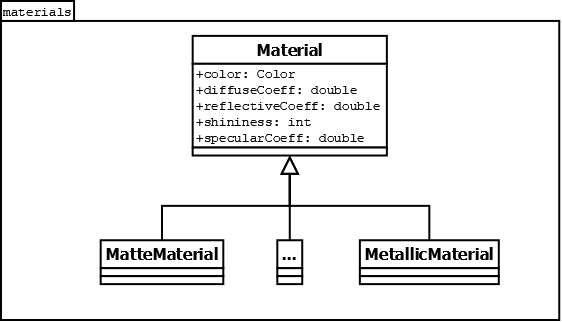
\includegraphics[width=0.75\textwidth]{diagrammes/package_materials.png}}
	
	\caption{Diagramme du package materials}
	\label{diagrammePackageMaterials}
\end{figure}
\FloatBarrier

Une classe mère Material permet de définir un matériau complètement arbitrairement. Toutes les caractéristiques peuvent être choisies comme on le souhaite. C'est cette classe qu'utilise le parser de fichier POV lorsqu'il doit construire un matériau à partir de ce qu'il rencontre dans le fichier POV donné en entrée.\\
Différentes classes héritent ensuite de cette classe mère afin de définir des catégories de matériau avec des propriétés fixées. Ces classes sont cependant devenues obsolètes après la finition du parser qui ne peut constuire que des matériaux arbitraires.


\end{document}